\chapter{如何对应敏捷与CMMI} % Introduction chapter suppressed from the table of contents

\hypertarget{ux5982ux4f55ux5bf9ux5e94ux654fux6377ux539fux5219}{%
\section{如何对应敏捷原则}\label{ux5982ux4f55ux5bf9ux5e94ux654fux6377ux539fux5219}}

下面借用前面提过的ACP 原则,看如何对应:

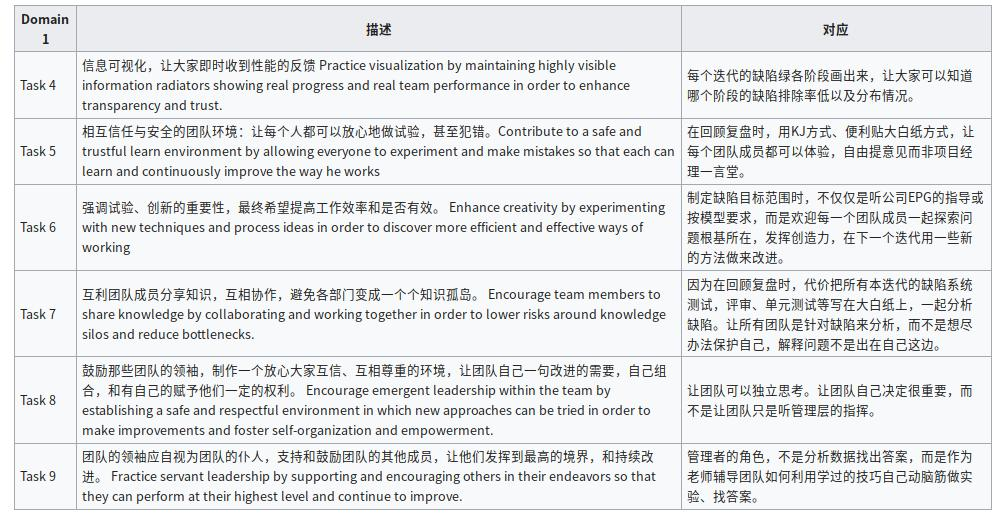
\includegraphics[width=10cm]{Screenshotfrom2022-01-24-1.jpg}

\hypertarget{ux5982ux4f55ux5bf9ux5e94-cmmi-ml4-ux8981ux6c42}{%
\section{如何对应 CMMI ML4
要求}\label{ux5982ux4f55ux5bf9ux5e94-cmmi-ml4-ux8981ux6c42}}

\hypertarget{mpm-4.4-ux4f7fux7528ux7edfux8ba1ux4e0eux5176ux4ed6ux91cfux5316ux6280ux672fux6765ux5efaux7acbux548cux5206ux6790ux8fc7ux7a0bux6027ux80fdux6a21ux578bux5e76ux4fddux6301ux66f4ux65b0use-statistical-and-other-quantitative-techniques-to-develop-and-analyze-process-performance-models-and-keep-them-updated.}{%
\subsection{MPM 4.4
使用统计与其他量化技术来建立和分析过程性能模型并保持更新。Use
statistical and other quantitative techniques to develop and analyze
process performance models and keep them
updated.}\label{mpm-4.4-ux4f7fux7528ux7edfux8ba1ux4e0eux5176ux4ed6ux91cfux5316ux6280ux672fux6765ux5efaux7acbux548cux5206ux6790ux8fc7ux7a0bux6027ux80fdux6a21ux578bux5e76ux4fddux6301ux66f4ux65b0use-statistical-and-other-quantitative-techniques-to-develop-and-analyze-process-performance-models-and-keep-them-updated.}}

其他必需信息 Additional Required Information

\begin{description}
\tightlist
\item[]
PPM 过程性能模型:
\end{description}

\begin{itemize}
\tightlist
\item
  是根据历史过程性能数据(如过程性能基线中包含的数据)开发的

  \begin{itemize}
  \tightlist
  \item
    依据每一个过程需求评审,开发,等系统导出数据,依据数据中的缺陷建立的模型
  \end{itemize}
\item
  以可度量的属性值和术语描述、描绘变动或对其进行建模

  \begin{itemize}
  \tightlist
  \item
    有一个度量定义表,蒙特卡洛中的变量定义在度量定义表中定义;变量与预测结果都有分布
  \end{itemize}
\item
  预测中间或最终过程性能

  \begin{itemize}
  \tightlist
  \item
    蒙特卡洛可以预测出QPPO范围与过程(如需求评审)缺陷范围
  \end{itemize}
\item
  估算预测结果的预期范围和变动

  \begin{itemize}
  \tightlist
  \item
    蒙特卡洛预测出中间或最终过程QPPO的预期范围和变动
  \end{itemize}
\item
  包含至少一个表示与子过程相关的可控输入的可度量属性

  \begin{itemize}
  \tightlist
  \item
    可控因素:各阶段的评审方法(如,用走查 或 审查)
  \end{itemize}
\end{itemize}

\begin{itemize}
\tightlist
\item
  Establish PPM - Monte Carlo analysis
\item
  Validate PPM - build PPM using historical iteration defect escape
  data, check and calibrate with the recent iteration defect results
\item
  Review PPM with affected stakeholders - whole team review in Sprint
  retrospective
\item
  Revise PPM - team review and revise (if needed) the PPM using the
  current Sprint defect data in Sprint retrospective
\end{itemize}

\hypertarget{mpm-4.5-ux4f7fux7528ux7edfux8ba1ux4e0eux5176ux4ed6ux91cfux5316ux6280ux672fux6765ux786eux5b9aux6216ux9884ux6d4bux8d28ux91cfux4e0eux8fc7ux7a0bux6027ux80fdux76eeux6807ux7684ux5b9eux73b0ux60c5ux51b5use-statistical-and-other-quantitative-techniques-to-determine-or-predict-achievement-of-quality-and-process-performance-objectives.}{%
\subsection{MPM 4.5
使用统计与其他量化技术来确定或预测质量与过程性能目标的实现情况Use
statistical and other quantitative techniques to determine or predict
achievement of quality and process performance
objectives.}\label{mpm-4.5-ux4f7fux7528ux7edfux8ba1ux4e0eux5176ux4ed6ux91cfux5316ux6280ux672fux6765ux786eux5b9aux6216ux9884ux6d4bux8d28ux91cfux4e0eux8fc7ux7a0bux6027ux80fdux76eeux6807ux7684ux5b9eux73b0ux60c5ux51b5use-statistical-and-other-quantitative-techniques-to-determine-or-predict-achievement-of-quality-and-process-performance-objectives.}}

\begin{itemize}
\tightlist
\item
  分析选定过程的变动和稳定性并解决缺陷

  \begin{itemize}
  \tightlist
  \item
    使用了方差分析和控制图
  \item
    通过趋势图,控制图判断历史数据是否作为基线,保证模型的稳定性。详见基线PPB截图。
  \item
    对各种方法进行方差分析,识别是否有显著区分
  \end{itemize}
\item
  实施必要的行动来解决在实现质量与过程性能目标方面的缺陷

  \begin{itemize}
  \tightlist
  \item
    P4 系统缺陷密度波动范围很广, 暂时不能预测,先对团队培训过程
  \end{itemize}
\item
  使用经数据校准并已确认的过程性能模型来评估质量与过程性能目标的实现进度

  \begin{itemize}
  \tightlist
  \item
    使用过程性能模型来预测下一轮冲刺的各阶段缺陷密度范围
  \end{itemize}
\item
  识别和管理与实现质量与过程性能目标有关的风险

  \begin{itemize}
  \tightlist
  \item
    利用PPM预测下一轮达到目标范围的概率
  \end{itemize}
\item
  记录并传达分析结果、决策以及确定的行动

  \begin{itemize}
  \tightlist
  \item
    把以上记录在量化项目管理计划
  \end{itemize}
\end{itemize}

\hypertarget{mpm-4.1-ux4f7fux7528ux7edfux8ba1ux4e0eux5176ux4ed6ux91cfux5316ux6280ux672fux6765ux5236ux5b9aux6301ux7eedux66f4ux65b0ux5e76ux4f20ux8fbeux53efux8ffdux6eafux5230ux4e1aux52a1ux76eeux6807ux7684ux8d28ux91cfux4e0eux8fc7ux7a0bux6027ux80fdux76eeux6807use-statistical-and-other-quantitative-techniques-to-develop-keep-updated-and-communicate-quality-and-process-performance-objectives-that-are-traceable-to-business-objectives.}{%
\subsection{MPM 4.1
使用统计与其他量化技术来制定、持续更新并传达可追溯到业务目标的质量与过程性能目标Use
statistical and other quantitative techniques to develop, keep updated,
and communicate quality and process performance objectives that are
traceable to business
objectives.}\label{mpm-4.1-ux4f7fux7528ux7edfux8ba1ux4e0eux5176ux4ed6ux91cfux5316ux6280ux672fux6765ux5236ux5b9aux6301ux7eedux66f4ux65b0ux5e76ux4f20ux8fbeux53efux8ffdux6eafux5230ux4e1aux52a1ux76eeux6807ux7684ux8d28ux91cfux4e0eux8fc7ux7a0bux6027ux80fdux76eeux6807use-statistical-and-other-quantitative-techniques-to-develop-keep-updated-and-communicate-quality-and-process-performance-objectives-that-are-traceable-to-business-objectives.}}

\begin{itemize}
\tightlist
\item
  QPPO

  \begin{itemize}
  \tightlist
  \item
    Org: Use CC, Monte Carlo simulation, ANOVA, to estimate SMART QPPO
  \item
    Project: Use PPM, PPB to predict QPPO for the next Sprint
  \end{itemize}
\item
  Derive interim objectives to monitor progress

  \begin{itemize}
  \tightlist
  \item
    Project: Use PPM, to also predict Req review, Code review, UT defect
    density range for the next Sprint
  \end{itemize}
\item
  Determine and record risk

  \begin{itemize}
  \tightlist
  \item
    Use PPM to predict the \% of achieving QPPO
  \end{itemize}
\item
  Resolve conflicts among QPPOs

  \begin{itemize}
  \tightlist
  \item
    PPM use overall cost to optimize, can balance the conflict between
    quality (minimize ST / AT defects density) and productivity
    objective
  \end{itemize}
\end{itemize}

\hypertarget{plan-4.1-ux4f7fux7528ux7edfux8ba1ux4e0eux5176ux4ed6ux91cfux5316ux6280ux672fux6765ux5f00ux53d1ux9879ux76eeux8fc7ux7a0bux5e76ux4fddux6301ux66f4ux65b0ux4ee5ux5b9eux73b0ux8d28ux91cfux4e0eux8fc7ux7a0bux6027ux80fdux76eeux6807use-statistical-and-other-quantitative-techniques-to-develop-and-keep-the-project-processes-updated-to-enable-achievement-of-the-quality-and-process-performance-objectives.}{%
\subsection{PLAN 4.1
使用统计与其他量化技术来开发项目过程并保持更新,以实现质量与过程性能目标。Use
statistical and other quantitative techniques to develop and keep the
project processes updated to enable achievement of the quality and
process performance
objectives.}\label{plan-4.1-ux4f7fux7528ux7edfux8ba1ux4e0eux5176ux4ed6ux91cfux5316ux6280ux672fux6765ux5f00ux53d1ux9879ux76eeux8fc7ux7a0bux5e76ux4fddux6301ux66f4ux65b0ux4ee5ux5b9eux73b0ux8d28ux91cfux4e0eux8fc7ux7a0bux6027ux80fdux76eeux6807use-statistical-and-other-quantitative-techniques-to-develop-and-keep-the-project-processes-updated-to-enable-achievement-of-the-quality-and-process-performance-objectives.}}

\begin{itemize}
\tightlist
\item
  制定用于评价项目过程备选方案的准则

  \begin{itemize}
  \tightlist
  \item
    总成本最低。
  \end{itemize}
\item
  识别或开发可用来完成工作和实现目标的替代过程

  \begin{itemize}
  \tightlist
  \item
    模型中已进行体现,通过不同的评审方法互相替换。
  \end{itemize}
\item
  根据记录的评价标准分析和评价备选过程

  \begin{itemize}
  \tightlist
  \item
    参考蒙特卡洛Optimize 仿真选择最佳配搭。
  \end{itemize}
\item
  选择最符合准则的备选过程

  \begin{itemize}
  \tightlist
  \item
    同上,在模型中体现。
  \end{itemize}
\item
  评价无法实现项目的质量与过程性能目标的风险

  \begin{itemize}
  \tightlist
  \item
    利用PPM预测结果的分布,分析概率
  \end{itemize}
\end{itemize}


